\documentclass{report}
\usepackage[utf8]{inputenc}
\usepackage[T1]{fontenc}
\usepackage{graphicx}
\usepackage[croatian]{babel}
\graphicspath{{slike/}}
\usepackage{url}


\begin{document}
\title{Računalo}
\author{Ivan Gluhak}
\date{21.1.2023}
\maketitle
\tableofcontents
\listoffigures

\chapter{Namjena i cijena računala}
Računalo je namijenjeno za igranje igara. Sama cijena od 2737 eura opravdava tu namjenu.Najveći dio novaca je uložen u sami procesor i grafičku karticu kako bi se postigla najveća brzina samog računala, isto tako računalo je pogodno za poslovni rad kao i za izradu samih slika.
 
\chapter{Procesor}
Procesor Intel Core i9-14900K 
\\ Procesor koji je danas jedan od najboljih na tržištu.Pruža brzi rad te najbolje performanse u igrama.
\\Cijena: 780€
\\Izvor:  \url{https://www.instar-informatika.hr/procesor-intel-core-i9-14900k-24c32t-up-to-60ghz-36mb-lga1700-/218299/product/}
\begin{figure}[h]
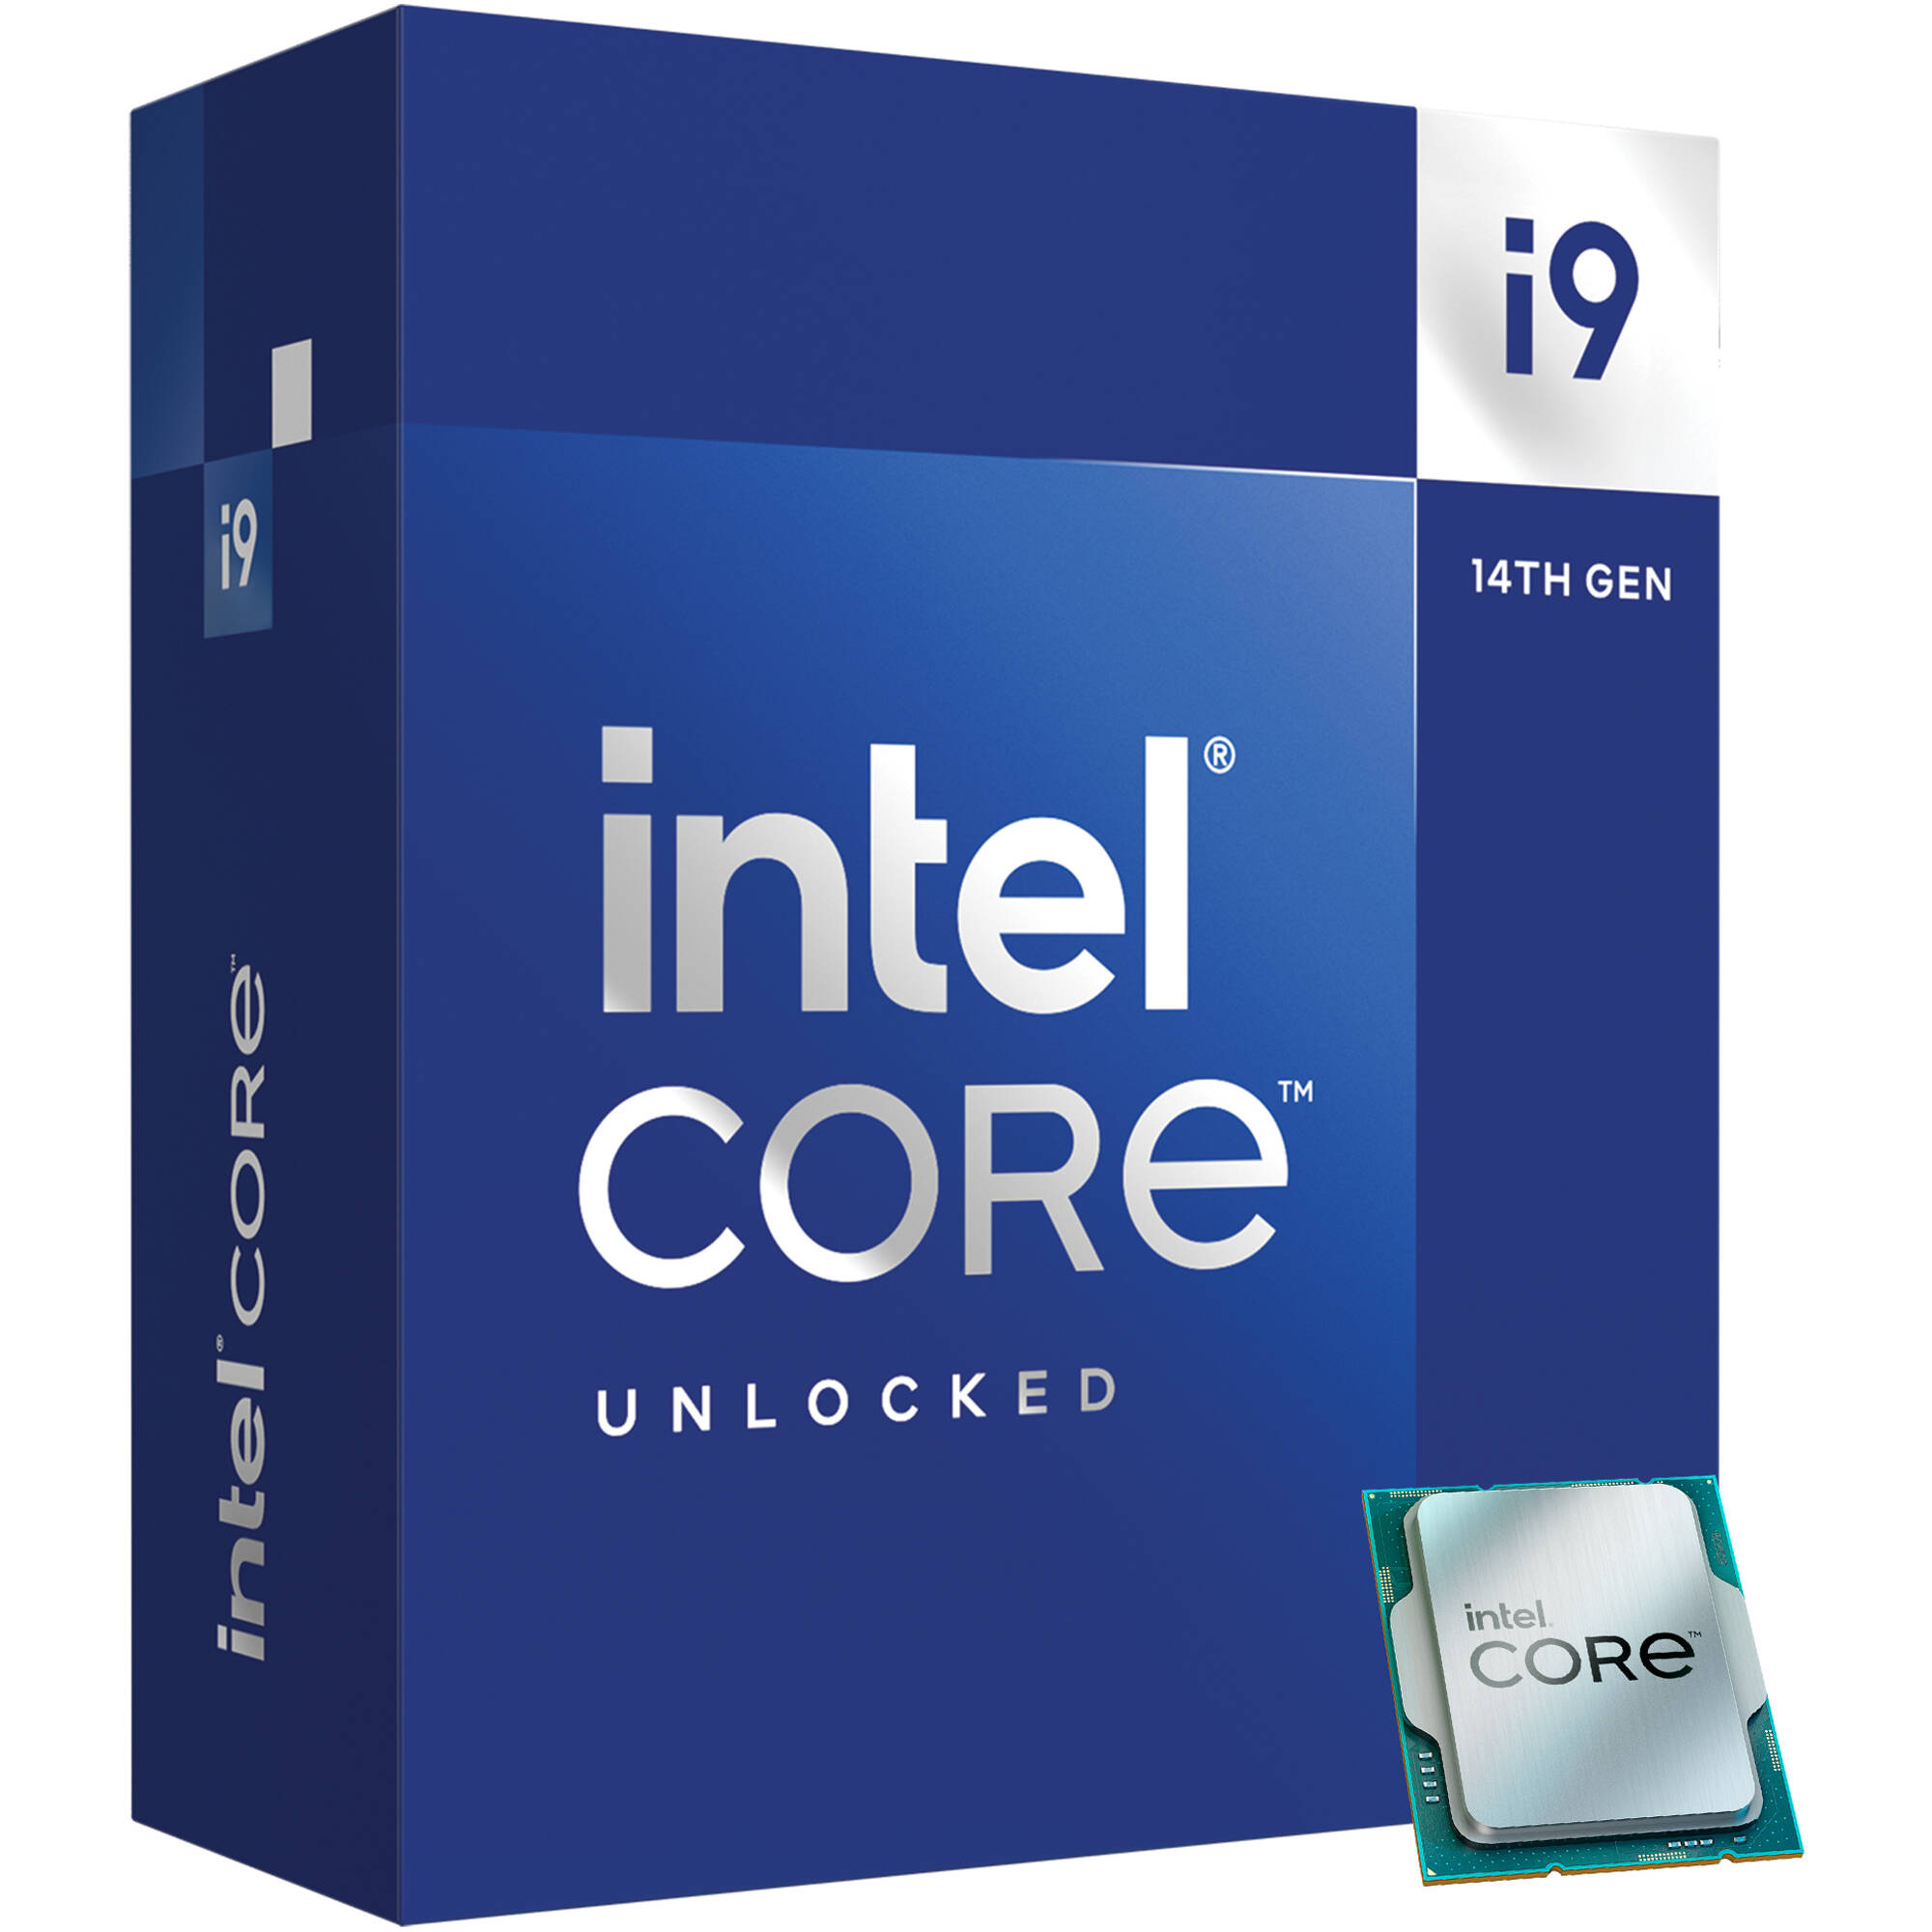
\includegraphics[width=8cm]{slike/procesor.jpg}
\caption{Intel Core i9}
\end{figure}

\chapter{Matična}
Matična ploča MSI MEG B550 UNIFY, AMD B550, ATX, AM4
\\Odabrao sam ovu matičnu ploču zbog pružanja najboljih performansi ali isto tako i cijene. Podržava razne procesore te isto tako sadrži wifi koji pruža brzi prijenos podataka
\\Cijena: 320€
\\Izvor:  \url{https://www.links.hr/hr/maticna-ploca-msi-meg-b550-unify-amd-b550-atx-am4-010502083}
\begin{figure}[h]
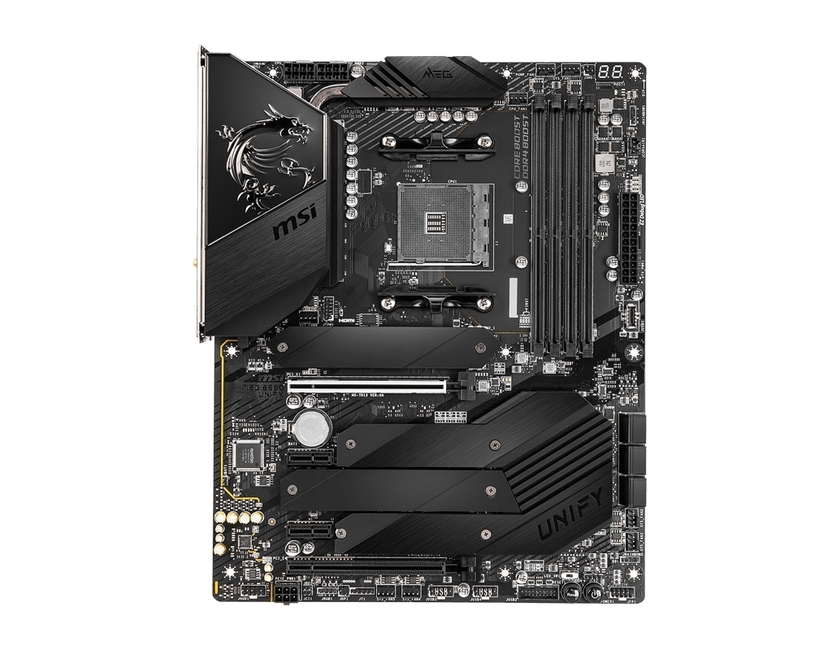
\includegraphics[width=7cm]{slike/maticna.jpg}
\caption{MSI MEG B550}
\end{figure}

\chapter{Grafička}
Asus TUF-RTX3060TI, 8GB DDR6X
\\Ova grafička kartica pruža jedne od najboljih performansi ali isto tako i sliku.Savršena za gameing ali i za poslovan rad na računalu ili izradu slika.
\\Cijena: 460€
\\Izvor:  \url{https://www.nabava.net/graficke-kartice/asus-tuf-rtx3060ti-o8gd6x-gaming-cijena-8gb-ddr6x-435957581}
\begin{figure}[h]
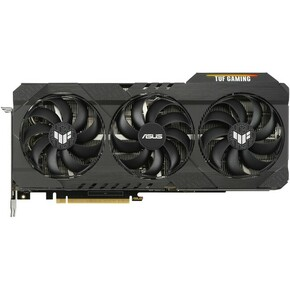
\includegraphics[width=8cm]{slike/graficka.jpg}
\caption{ASUS TUF RTX 3060}
\end{figure}

\chapter{RAM}
Memorija Corsair Vengeance RGB Pro, 32GB (2x16GB), DDR4 3600MHz
\\32 GB radne memorije je dovoljno za brzi i stabilan rad računala. Posjeduje brzinu od 3600 MHz te sami RGB uređaj za bolji izgled računala 
\\Cijena: 120€
\\Izvor:  \url{https://www.instar-informatika.hr/memorija-corsair-vengeance-rgb-pro-32gb-2x16gb-ddr4-3600mhz-cl18/216133/product/}
\begin{figure}[h]
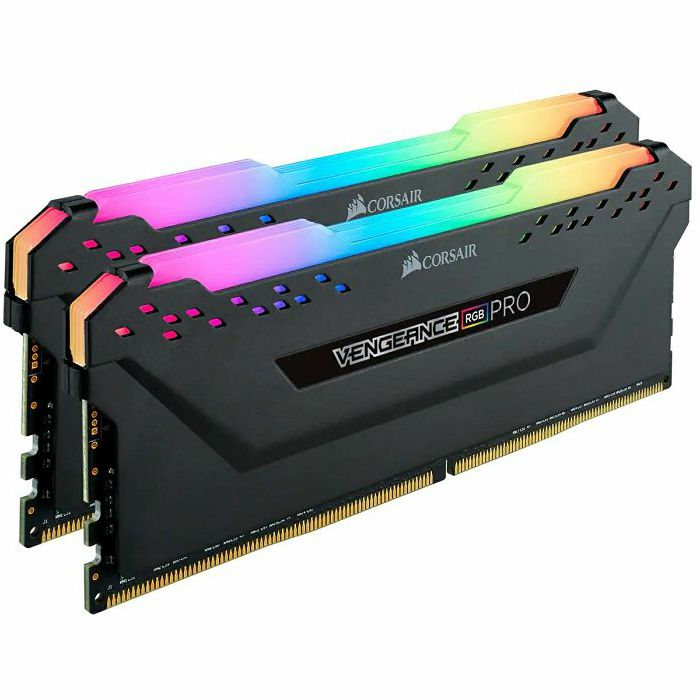
\includegraphics[width=8cm]{slike/ram.jpg}
\caption{Corsair Vengeance RGB Pro 3600MHz}
\end{figure}

\chapter{Trajna memorija}
SSD Crucial T700 Heatsink, 1TB, M.2 NVMe PCIe Gen5, R11700/W9500
SSD Crucial pruža veliku količinu prostora te izuzetnu brzinu.Aplikacije će sa lakoćom pokretati.
\\Cijena: 263€
\\Izvor:  \url{https://www.instar-informatika.hr/ssd-crucial-t700-heatsink-1tb-m2-nvme-pcie-gen5-r11700w9500/165420/product/}
\begin{figure}[h]
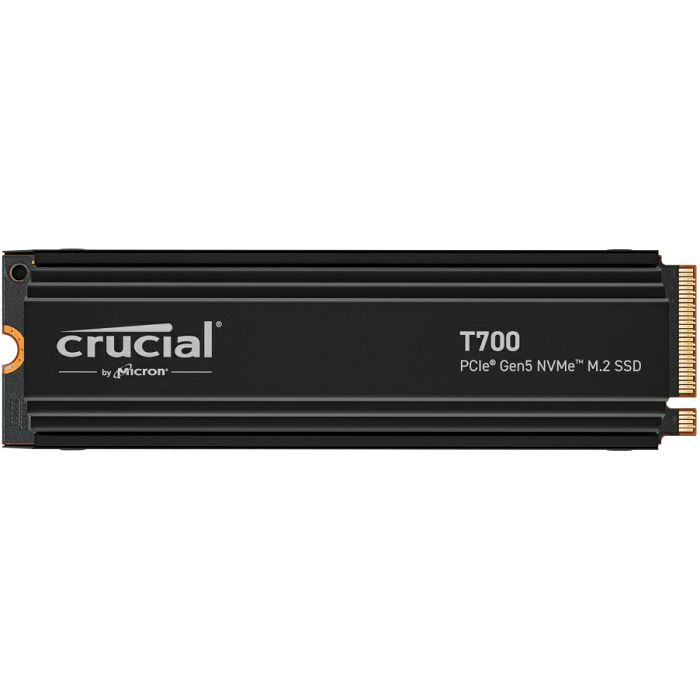
\includegraphics[width=8cm]{slike/ssd.jpg}
\caption{Crucial T700}
\end{figure}

\chapter{Kućište}
Thermaltake CA-1X3-00M6WN-00
\\ Thermaltake pruža najlijepsi izgled , laku dostupnost komponentama ali isto tako i prozračnost za samo hlađenje računala.
\\Cijena: 105€
\\Izvor:  \url{https://www.conrad.hr/hr/p/thermaltake-ca-1x3-00m6wn-00-midi-tower-kuciste-za-igrace-racunalo-bijela-3-predinstalirana-led-ventilatora-bocni-proz-2799625.html}
\begin{figure}[h]
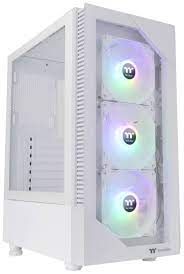
\includegraphics[width=5cm]{slike/kuciste.jpg}
\caption{Thermaltake}
\end{figure}

\chapter{Napajanje}
Napajanje 850W, THERMALTAKE Toughpower GF3 ARGB 850W Gold, ATX 3.0, 140mm vent., modularno, 80+ Gold
\\Napajanje Thermaltake GF3 pruža dovoljnu količinu energije za rad računala.Certifikat 80+ Gold osigurava energetsku učinkovitost.Ima ugrađeni RGB što daje samo lijepotu računalu
\\Cijena: 200€
\begin{figure}[h]
Izvor:  \url{https://www.links.hr/hr/napajanje-850w-thermaltake-toughpower-gf3-argb-850w-gold-atx-3-0-140mm-vent-modularno-80-gold-010507121}
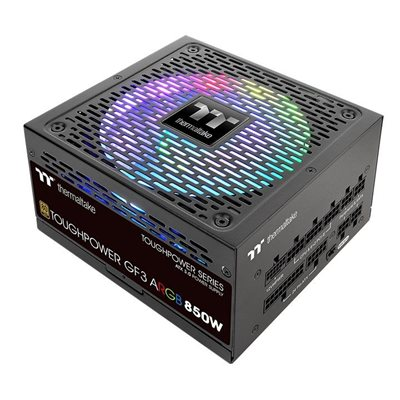
\includegraphics[width=8cm]{slike/napajanje.jpg}
\caption{Thermaltake GF3}
\end{figure}


\chapter{Monitor}
Monitor 24" AOC 24G2SPU, IPS, FHD, 165Hz
\\AOC pruža osviježavanje slike od 165 Hz što pruža veliki ugođaj tokom igranje igara.
\\Cijena: 225€
\\Izvor:  \url{https://www.sancta-domenica.hr/racunala-i-periferija/monitori-pc/monitor-aoc-24-24g2spu-fhd-dp-2xhdmi-has-165hz-4xusb3-0.html}
\begin{figure}[h]
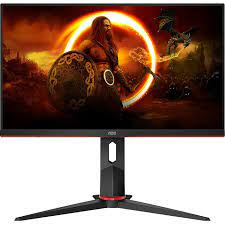
\includegraphics[width=8cm]{slike/monitor.jpg}
\caption{AOC Monitor}
\end{figure}

\chapter{Tipkovnica}
WHITE SHARK gaming tipkovnica GK-2201
\\White Shark tipkovnica pruža dobar omjer cijene i kvalitete. Brzi odaziv na pritisak te sama boja i RGB osvijetljenje ulijepsavaju samo racunalo.
\\Cijena: 30€
\\Izvor:  \url{https://hyperlift.hr/hr/tipkovnice/white-shark-tipkovnica-gk2201-ronin-bijela-hr}
\begin{figure}[h]
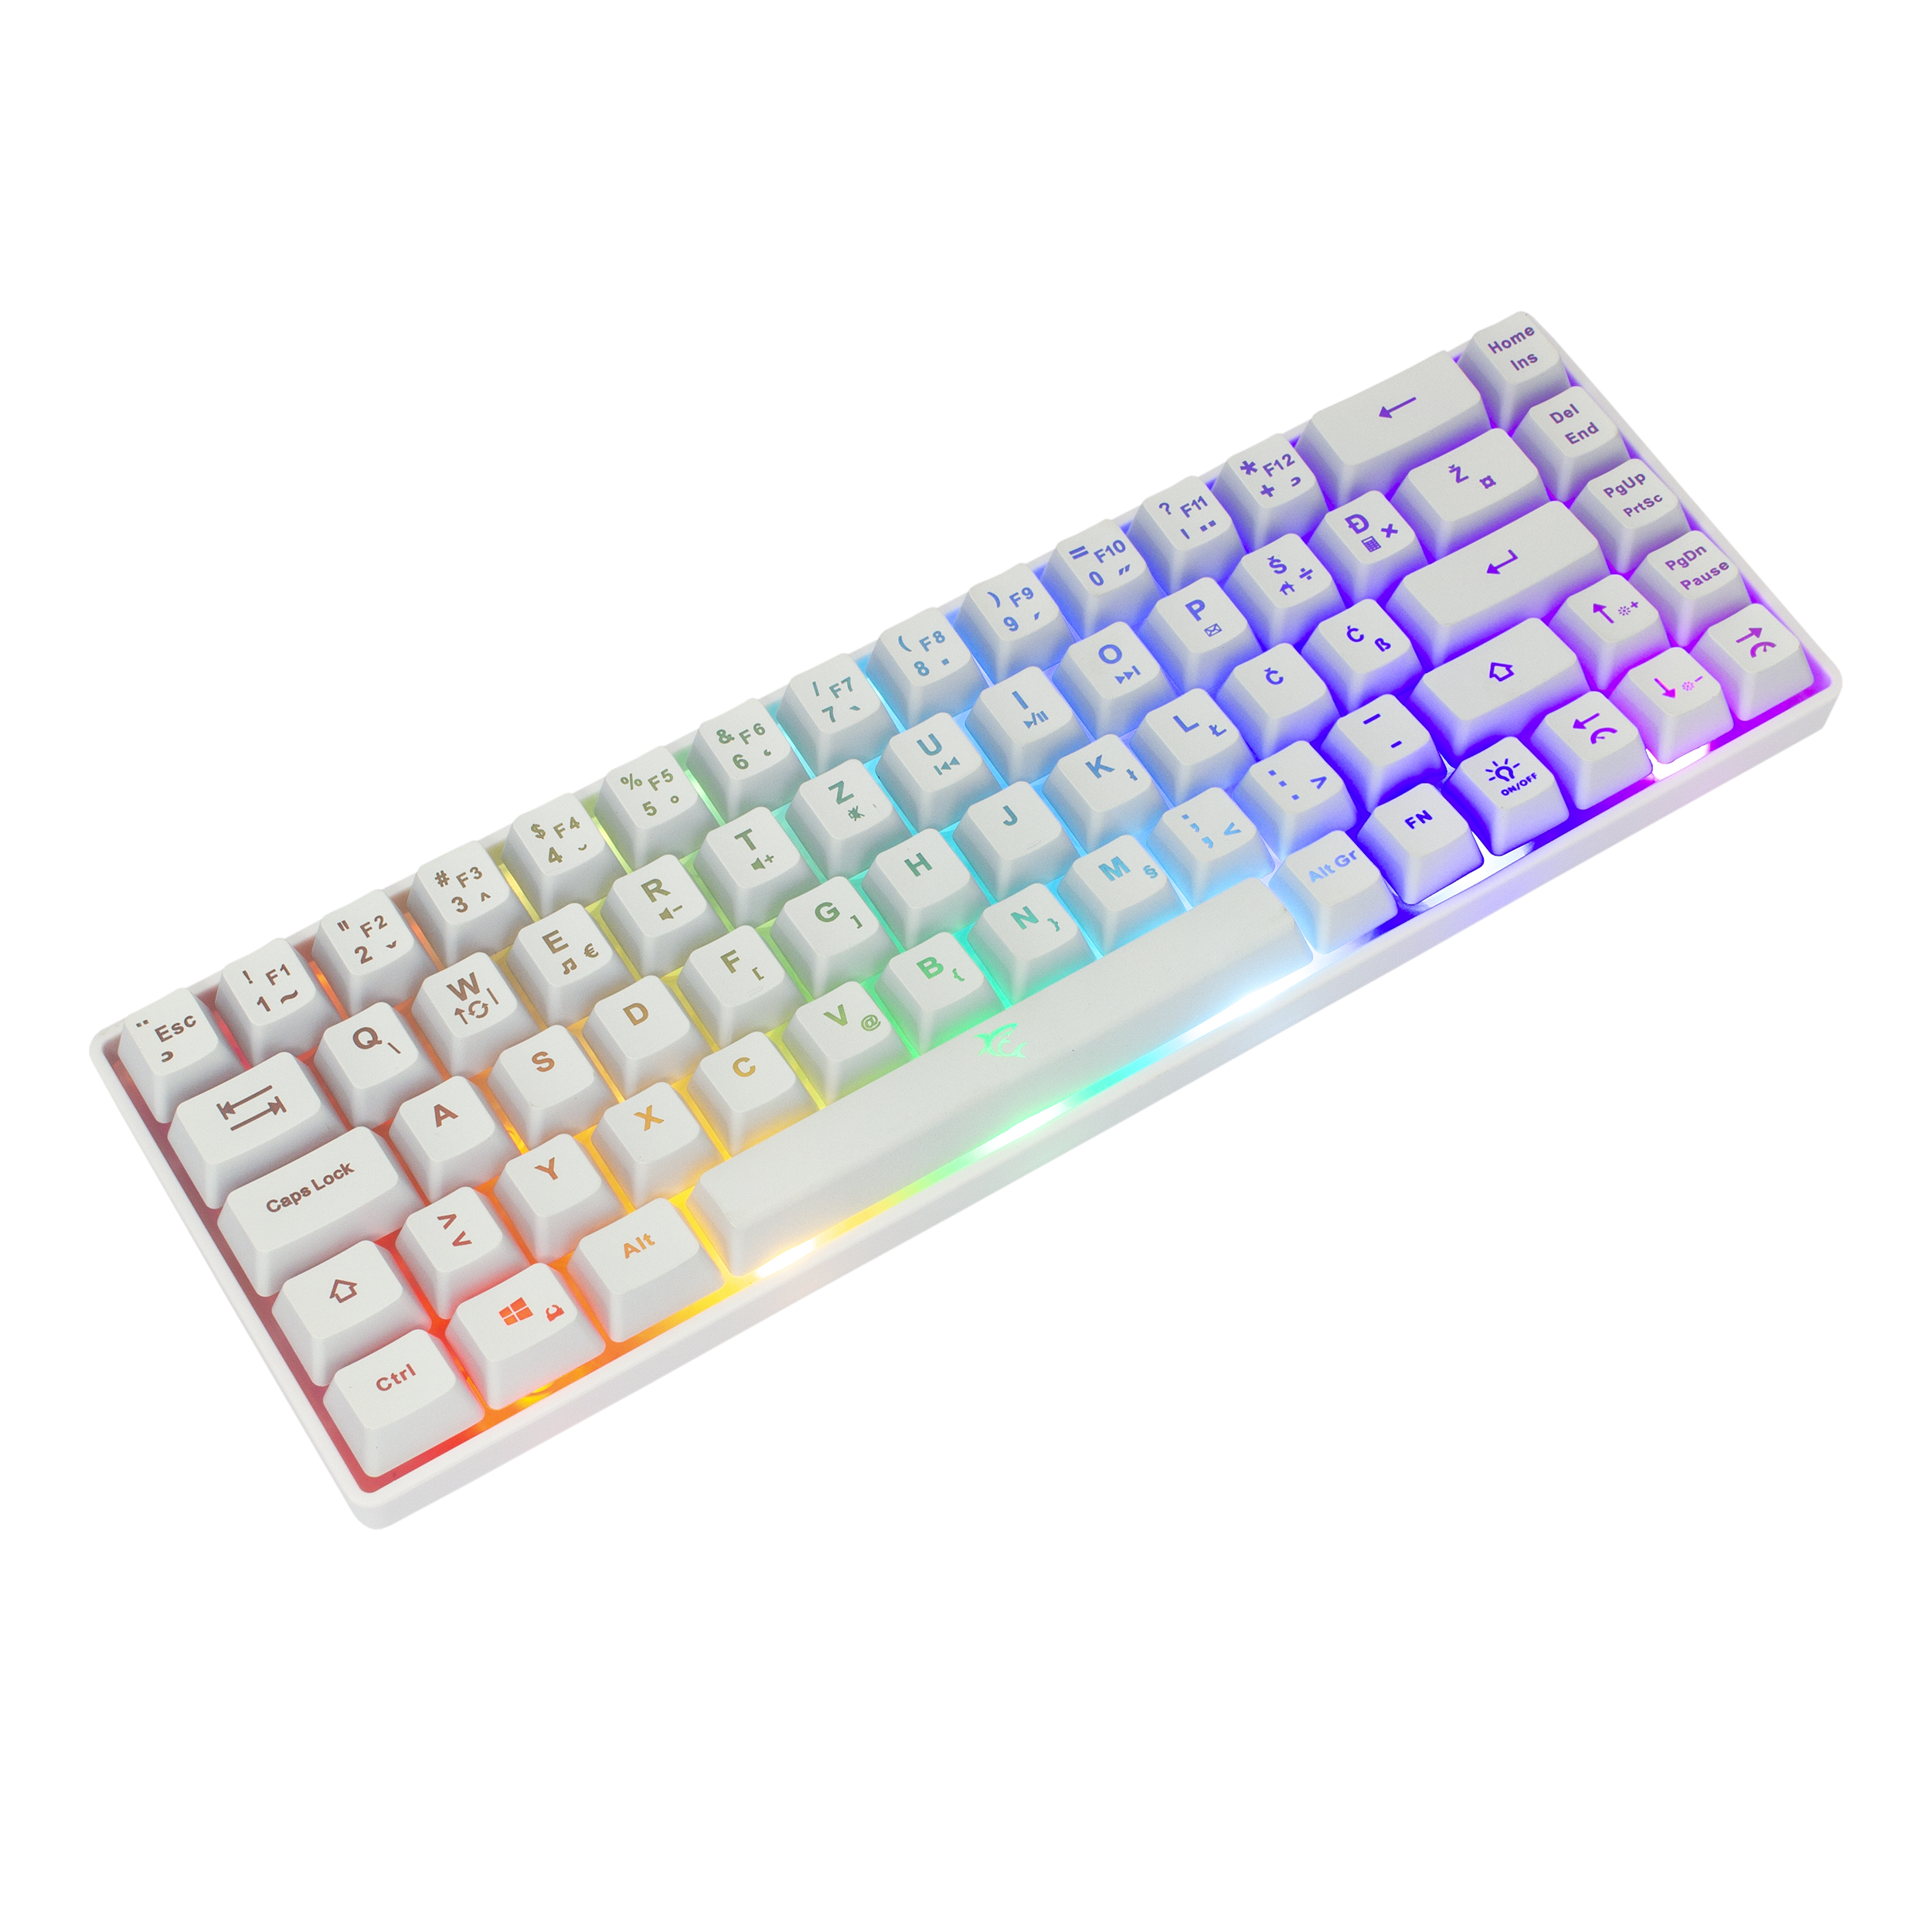
\includegraphics[width=8cm]{slike/tipkovnica.jpg}
\caption{White Shark GK-2201}
\end{figure}

\chapter{Miš}
Logitech G Pro X Superlight 
\\Logitech G pro pruža veliku prostranost jer posjeduje bežići prijenos.Brz odaziv na tipke te sami ugođaj pri korištenju su odlični.
\\Cijena: 160€
\\Izvor:  \url{https://www.links.hr/hr/mis-logitech-pro-x-superlight-bezicni-opticki-25600dpi-bijeli-usb-101500580}
\begin{figure}[h]
\includegraphics[width=8cm]{slike/miš.jpg}
\caption{Logitech G Pro X Superlight}
\end{figure}

\chapter{Slušalice}
Slušalice Razer BlackShark V2 X
\\Razer BlackShark V2 X su lagane te imaju najveću udobnost.Koriste najnovije tehnologije kako bi ugođaj i zvuk tokom igranja igara bio na najvećem nivou
\\Cijena: 74€
\\Izvor:  \url{https://www.instar-informatika.hr/slusalice-razer-blackshark-v2-x-zicane-gaming-71-mikrofon-over-e/96560/product/}
\begin{figure}[h]
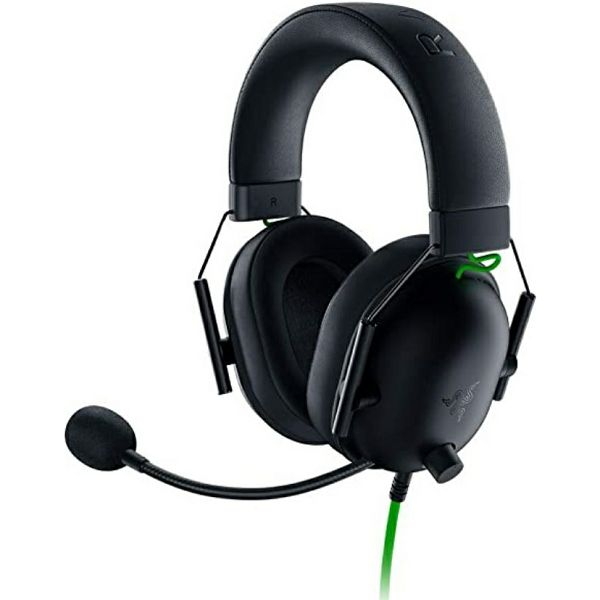
\includegraphics[width=8cm]{slike/slusalice.jpg}
\caption{Razer BlackShark V2 X}
\end{figure}

\end{document}